\section{Experiments}
\begin{frame}{Overview}
    
\end{frame}
\begin{frame}{Measurements}
    \twocol{
        \vspace{-0.5cm}
        \begin{figure}
    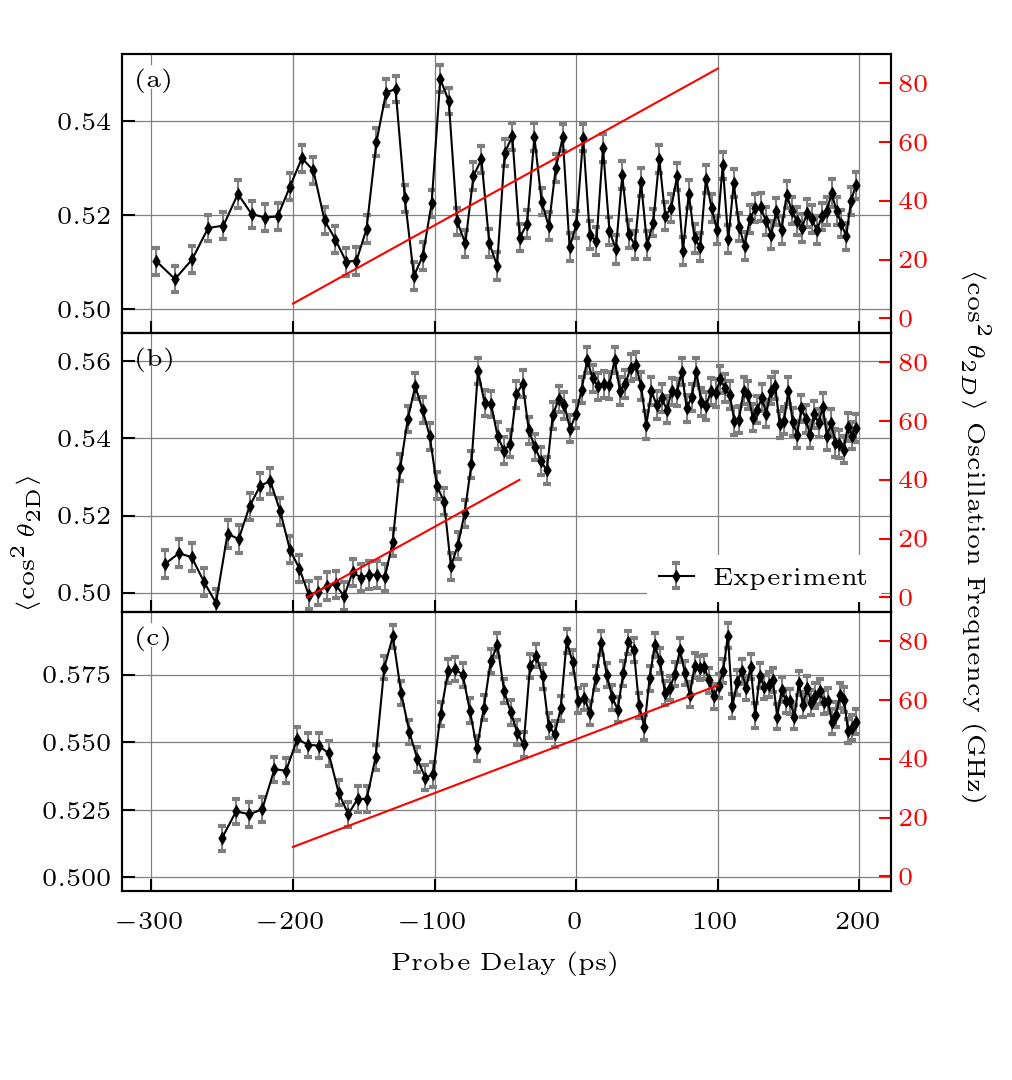
\includegraphics[width=\linewidth]{figures/cs2-ocs-comparison_v3.png}
  \end{figure}
    }{
        \begin{block}{a) $\mathrm{CS}_2$ with fast centrifuge}
            \begin{itemize}
                \item spinning way above the wall (around $20\,\mathrm{GHz}$)
            \end{itemize}
        \end{block}
        \begin{block}{b) $\mathrm{OCS}$ with fast centrifuge}
            \begin{itemize}
                \item spinning worse than $\mathrm{CS}_2$
                \item different lower envelope
            \end{itemize}
        \end{block}
        \begin{block}{c) $\mathrm{OCS}$ with slower centrifuge}
            \begin{itemize}
                \item slower acceleration spins molecule further
            \end{itemize}
        \end{block}
    }
    \begin{itemize}
        \item for all droplet measurements the amplitude decreases in the middle of the pulse
    \end{itemize}
\end{frame}
\begin{frame}{Measurements}
    \twocol{
        \vspace{-0.5cm}
        \begin{figure}
    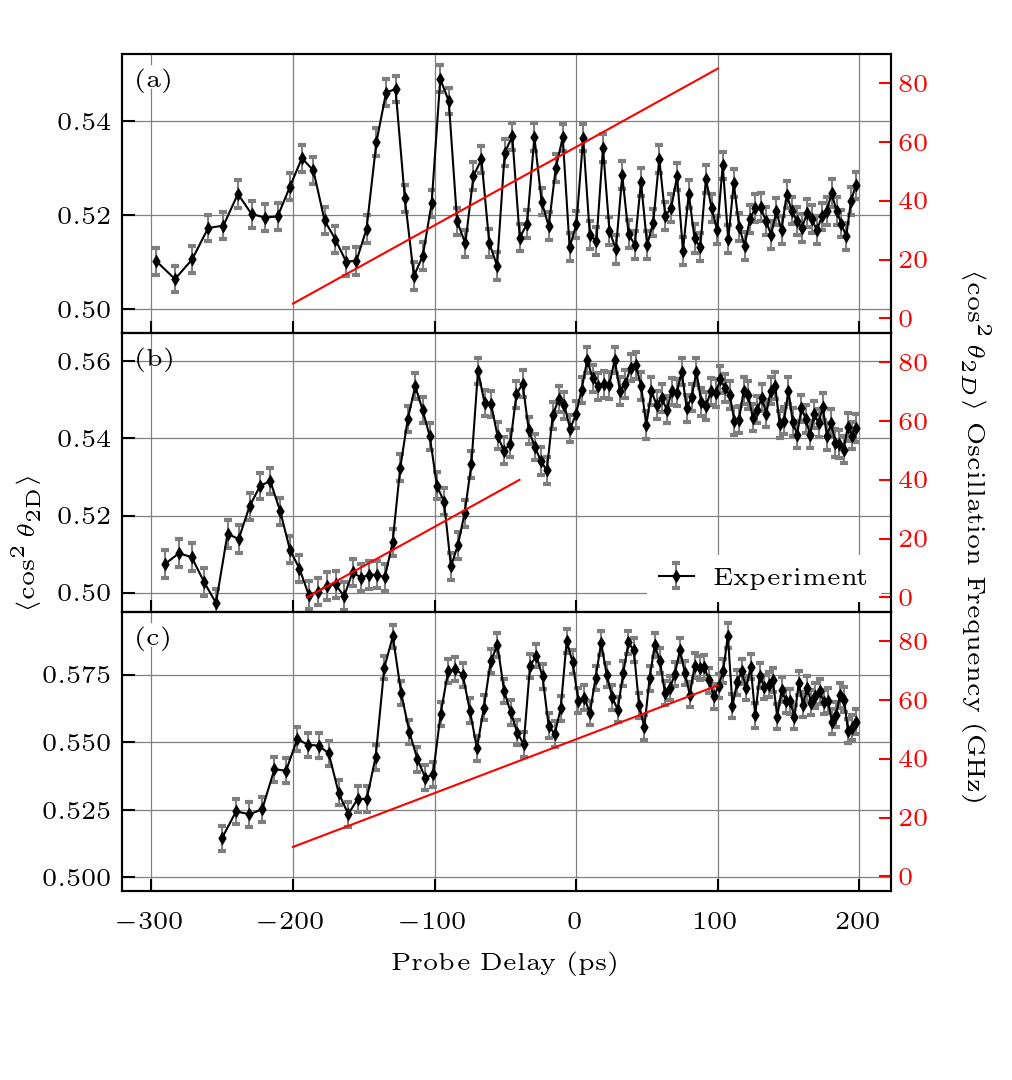
\includegraphics[width=\linewidth]{figures/cs2-ocs-comparison_v3.png}
  \end{figure}
    }{
        \begin{bigidea}{Important Detail}
            \begin{itemize}
            \item for all droplet measurements the amplitude decreases in the middle of the pulse
            \item this appears to be at different frequencies for different molecules
            \end{itemize}
        \end{bigidea}
    }
\end{frame}